% Options for packages loaded elsewhere
\PassOptionsToPackage{unicode}{hyperref}
\PassOptionsToPackage{hyphens}{url}
%
\documentclass[
  english,
  man]{apa6}
\author{\phantom{0}}
\date{}

\usepackage{amsmath,amssymb}
\usepackage{lmodern}
\usepackage{iftex}
\ifPDFTeX
  \usepackage[T1]{fontenc}
  \usepackage[utf8]{inputenc}
  \usepackage{textcomp} % provide euro and other symbols
\else % if luatex or xetex
  \usepackage{unicode-math}
  \defaultfontfeatures{Scale=MatchLowercase}
  \defaultfontfeatures[\rmfamily]{Ligatures=TeX,Scale=1}
\fi
% Use upquote if available, for straight quotes in verbatim environments
\IfFileExists{upquote.sty}{\usepackage{upquote}}{}
\IfFileExists{microtype.sty}{% use microtype if available
  \usepackage[]{microtype}
  \UseMicrotypeSet[protrusion]{basicmath} % disable protrusion for tt fonts
}{}
\makeatletter
\@ifundefined{KOMAClassName}{% if non-KOMA class
  \IfFileExists{parskip.sty}{%
    \usepackage{parskip}
  }{% else
    \setlength{\parindent}{0pt}
    \setlength{\parskip}{6pt plus 2pt minus 1pt}}
}{% if KOMA class
  \KOMAoptions{parskip=half}}
\makeatother
\usepackage{xcolor}
\IfFileExists{xurl.sty}{\usepackage{xurl}}{} % add URL line breaks if available
\IfFileExists{bookmark.sty}{\usepackage{bookmark}}{\usepackage{hyperref}}
\hypersetup{
  pdflang={en-EN},
  hidelinks,
  pdfcreator={LaTeX via pandoc}}
\urlstyle{same} % disable monospaced font for URLs
\usepackage{longtable,booktabs,array}
\usepackage{calc} % for calculating minipage widths
% Correct order of tables after \paragraph or \subparagraph
\usepackage{etoolbox}
\makeatletter
\patchcmd\longtable{\par}{\if@noskipsec\mbox{}\fi\par}{}{}
\makeatother
% Allow footnotes in longtable head/foot
\IfFileExists{footnotehyper.sty}{\usepackage{footnotehyper}}{\usepackage{footnote}}
\makesavenoteenv{longtable}
\usepackage{graphicx}
\makeatletter
\def\maxwidth{\ifdim\Gin@nat@width>\linewidth\linewidth\else\Gin@nat@width\fi}
\def\maxheight{\ifdim\Gin@nat@height>\textheight\textheight\else\Gin@nat@height\fi}
\makeatother
% Scale images if necessary, so that they will not overflow the page
% margins by default, and it is still possible to overwrite the defaults
% using explicit options in \includegraphics[width, height, ...]{}
\setkeys{Gin}{width=\maxwidth,height=\maxheight,keepaspectratio}
% Set default figure placement to htbp
\makeatletter
\def\fps@figure{htbp}
\makeatother
\setlength{\emergencystretch}{3em} % prevent overfull lines
\providecommand{\tightlist}{%
  \setlength{\itemsep}{0pt}\setlength{\parskip}{0pt}}
\setcounter{secnumdepth}{-\maxdimen} % remove section numbering
% Make \paragraph and \subparagraph free-standing
\ifx\paragraph\undefined\else
  \let\oldparagraph\paragraph
  \renewcommand{\paragraph}[1]{\oldparagraph{#1}\mbox{}}
\fi
\ifx\subparagraph\undefined\else
  \let\oldsubparagraph\subparagraph
  \renewcommand{\subparagraph}[1]{\oldsubparagraph{#1}\mbox{}}
\fi
% Manuscript styling
\usepackage{upgreek}
\captionsetup{font=singlespacing,justification=justified}

% Table formatting
\usepackage{longtable}
\usepackage{lscape}
% \usepackage[counterclockwise]{rotating}   % Landscape page setup for large tables
\usepackage{multirow}		% Table styling
\usepackage{tabularx}		% Control Column width
\usepackage[flushleft]{threeparttable}	% Allows for three part tables with a specified notes section
\usepackage{threeparttablex}            % Lets threeparttable work with longtable

% Create new environments so endfloat can handle them
% \newenvironment{ltable}
%   {\begin{landscape}\centering\begin{threeparttable}}
%   {\end{threeparttable}\end{landscape}}
\newenvironment{lltable}{\begin{landscape}\centering\begin{ThreePartTable}}{\end{ThreePartTable}\end{landscape}}

% Enables adjusting longtable caption width to table width
% Solution found at http://golatex.de/longtable-mit-caption-so-breit-wie-die-tabelle-t15767.html
\makeatletter
\newcommand\LastLTentrywidth{1em}
\newlength\longtablewidth
\setlength{\longtablewidth}{1in}
\newcommand{\getlongtablewidth}{\begingroup \ifcsname LT@\roman{LT@tables}\endcsname \global\longtablewidth=0pt \renewcommand{\LT@entry}[2]{\global\advance\longtablewidth by ##2\relax\gdef\LastLTentrywidth{##2}}\@nameuse{LT@\roman{LT@tables}} \fi \endgroup}

% \setlength{\parindent}{0.5in}
% \setlength{\parskip}{0pt plus 0pt minus 0pt}

% \usepackage{etoolbox}
\makeatletter
\patchcmd{\HyOrg@maketitle}
  {\section{\normalfont\normalsize\abstractname}}
  {\section*{\normalfont\normalsize\abstractname}}
  {}{\typeout{Failed to patch abstract.}}
\patchcmd{\HyOrg@maketitle}
  {\section{\protect\normalfont{\@title}}}
  {\section*{\protect\normalfont{\@title}}}
  {}{\typeout{Failed to patch title.}}
\makeatother
\shorttitle{SHORTTITLE}
\usepackage{csquotes}
\usepackage{float}
\usepackage{sectsty}
\usepackage{lscape}
\newcommand{\blandscape}{\begin{landscape}}
\newcommand{\elandscape}{\end{landscape}}
\ifXeTeX
  % Load polyglossia as late as possible: uses bidi with RTL langages (e.g. Hebrew, Arabic)
  \usepackage{polyglossia}
  \setmainlanguage[]{english}
\else
  \usepackage[main=english]{babel}
% get rid of language-specific shorthands (see #6817):
\let\LanguageShortHands\languageshorthands
\def\languageshorthands#1{}
\fi
\ifLuaTeX
  \usepackage{selnolig}  % disable illegal ligatures
\fi


\affiliation{\phantom{0}}

\begin{document}

\hypertarget{chapitre-4-utiliser-le-bmg-de-hedges-basuxe9-sur-luxe9cart-type-non-pooluxe9}{%
\section{\texorpdfstring{Chapitre 4 : Utiliser le \(\bm{g^*}\) de Hedges basé sur l'écart-type non poolé}{Chapitre 4 : Utiliser le \textbackslash bm\{g\^{}*\} de Hedges basé sur l'écart-type non poolé}}\label{chapitre-4-utiliser-le-bmg-de-hedges-basuxe9-sur-luxe9cart-type-non-pooluxe9}}

\begin{center}
\includegraphics[width=1.5\linewidth]{C:/Users/mdelacre/Documents/Github project/thesis/Chapitre 4/title} \end{center}

\begin{center}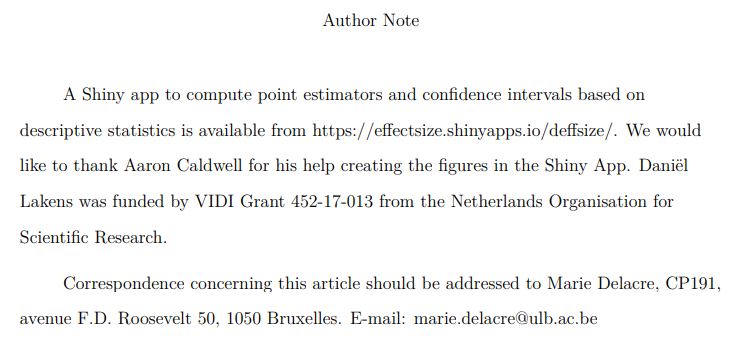
\includegraphics[width=1.5\linewidth]{C:/Users/mdelacre/Documents/Github project/thesis/Chapitre 4/authornote} \end{center}

\textbf{Commentaire} : l'article présenté dans ce chapitre n'a pas encore été accepté pour publication.

\newpage

Effect sizes are an important outcome of empirical research. Moving beyond decisions about statistical significance, there is a strong call for researchers to report and interpret effect sizes and associated confidence intervals. This practice is highly endorsed by the American Psychological Association (APA) and the American Educational Research Association (\textbf{association\_publication\_2010?}; \textbf{duran\_standards\_2006?}).

In ``between-subject'' designs where individuals are randomly assigned into one of two independent groups and group scores are compared based on their means, the dominant estimator of effect size is Cohen's \(d\), where the sample mean difference is divided by the pooled sample standard deviation (Peng et al., 2013; Shieh, 2013). This estimator is available in many statistical software packages, such as SPSS and Stata. However, computing the pooled sample standard deviation assumes that both sample variances are estimates of a common population variance, which is known as the homogeneity of variance assumption. It has been widely argued that there are many fields in psychology where this assumption is ecologically unlikely (Delacre et al., 2017; Erceg-Hurn \& Mirosevich, 2008; Grissom, 2000). The question how to deal with the assumption of equal variances has been widely explored in the context of hypothesis testing, and it is becoming increasingly common to by default report a \emph{t}-test that does not assume equal variances, such as Welch's \emph{t}-test.

However, the question which effect size to report when equal variances are not assumed has received less attention. One possible reason is that researchers have not found consensus on which of the available options should be used (\textbf{shieh\_confidence\_2013?}). Even within the very specific context of an estimate for the standardized sample mean difference there is little agreement about which estimator is the best choice. In this article, we will review the main candidates that have been proposed in the literature in the \emph{d} family of effect sizes, without (Cohen's \(d\), Glass's \(d\), Shieh's \(d\) and Cohen's \(d^*\)) and with correction for bias (Hedges' \(g\), Glass's \(g\), Shieh's \(g\) and Hedges' \(g^*\)). We provide an R package and Shiny app to compute relevant effect size measures and their confidence intervals.

Before reviewing the most important effect size measures in the \emph{d}-family, we will first list the different purposes effect size measures serve, and discuss the relationship between effect sizes, statistical, and practical significance. Based on a detailed description of the good properties an effect size measure should possess, we will evaluate these properties in the Monte Carlo simulations we performed to compare the different effect size estimators with correction for bias.

\hypertarget{three-purposes-of-effect-size-estimators}{%
\subsection{Three purposes of effect size estimators}\label{three-purposes-of-effect-size-estimators}}

The effect size is a measure of the magnitude of an effect. In the context of the comparison of two groups based on their means, when the null hypothesis is the absence of effect, \emph{d}-family effect size estimators estimate the magnitude of the differences between parameters of two populations groups are extracted from (e.g.~the mean; Peng \(\&\) Chen, 2014). Such a measure can be used for three different purposes.

First, effect size measures can be used for \emph{interpretative} purposes. They allow researchers to assess the practical significance of a result (i.e.~statements about the relevance of an effect in real life). In order to assess the meaningfulness of an effect, we should be able to relate this effect size estimate with behaviors/meaningful consequences in the real world (Andersen et al., 2007). This typically involves an analysis of the costs (determined by a specific context) and the benefits (in part determined by the size of the effect). It is important to remember an effect size is just a mathematical indicator of the magnitude of a difference, which depends on the way a variable is converted into numerical indicator. An effect size in itself is not a measure of the importance or the relevance of an effect for real life (even if benchmarks for small, medium, or large effect sizes might have contributed to such a misinterpretation; Stout
\(\&\) Ruble, 1995).

Second, effect size measures can be used for \emph{comparative} purposes. They allow researchers to assess the stability of results across designs, analyses, and sample sizes. This includes statistically comparing and combining the results from two or more studies in a meta-analysis.

Third, effect size measures can be used for \emph{inferential} purposes. Hypothesis tests and confidence intervals based on the same statistical quantity are directly related : if the area of the null hypothesis is out of the \((1-\alpha)\)-confidence interval, then the hypothesis test would also result in a \emph{p}-value below the nominal alpha level. At the same time, the interval provides extra information about the precision of the sample estimate for inferential purposes (\textbf{ellis\_essential\_2010?}; \textbf{altman\_why\_2005?}), and which effect sizes are excluded. The narrower the interval, the higher the precision, and the wider the confidence interval, the more the data lack precision. Effect size measures are also indirectly related to the hypothesis tests as effect sizes from previous studies can be used in an a-priori power analysis when planning a new study (\textbf{sullivan\_using\_2012?}; \textbf{lakens\_calculating\_2013?}; \textbf{stout\_assessing\_1995?}; \textbf{prentice\_when\_1992?}; \textbf{wilkinson\_statistical\_1999?}).

\hypertarget{inferential-properties-of-a-good-effect-size-estimator}{%
\subsection{Inferential properties of a good effect size estimator}\label{inferential-properties-of-a-good-effect-size-estimator}}

The empirical value of an estimator (called the \emph{estimate}) depends on the sample value. Different samples extracted from the same population will lead to different sample estimates of the population value. The \emph{sampling distribution} of the estimator is the distribution of all estimates, based on all possible samples of size \emph{n} extracted from one population. Studying the sampling distribution is useful, as it allows us to assess the qualities of an estimator. More specifically, three desirable properties a good estimator should possess for inferential purposes are : \emph{unbiasedness}, \emph{consistency} and \emph{efficiency} (Wackerly et al., 2008).

An estimator is unbiased if the distribution of estimates is centered around the true population parameter. On the other hand, an estimator is positively (or negatively) biased if the distribution is centered around a value that is higher (or lower) than the true population parameter (see Figure \ref{fig:BIAS}). In other words, examining the bias of an estimator tells us if estimates are on average accurate. The \emph{bias} of a point estimator \(\hat{\delta}\) can be computed as
\begin{equation} 
\delta_{bias}=E(\hat{\delta})-\delta
\label{eqn:BIAS}
\end{equation}
where \(E(\hat{\delta})\) is the expectation of the sampling distribution of the estimator and \(\delta\) is the true (population) parameter.

\begin{figure}
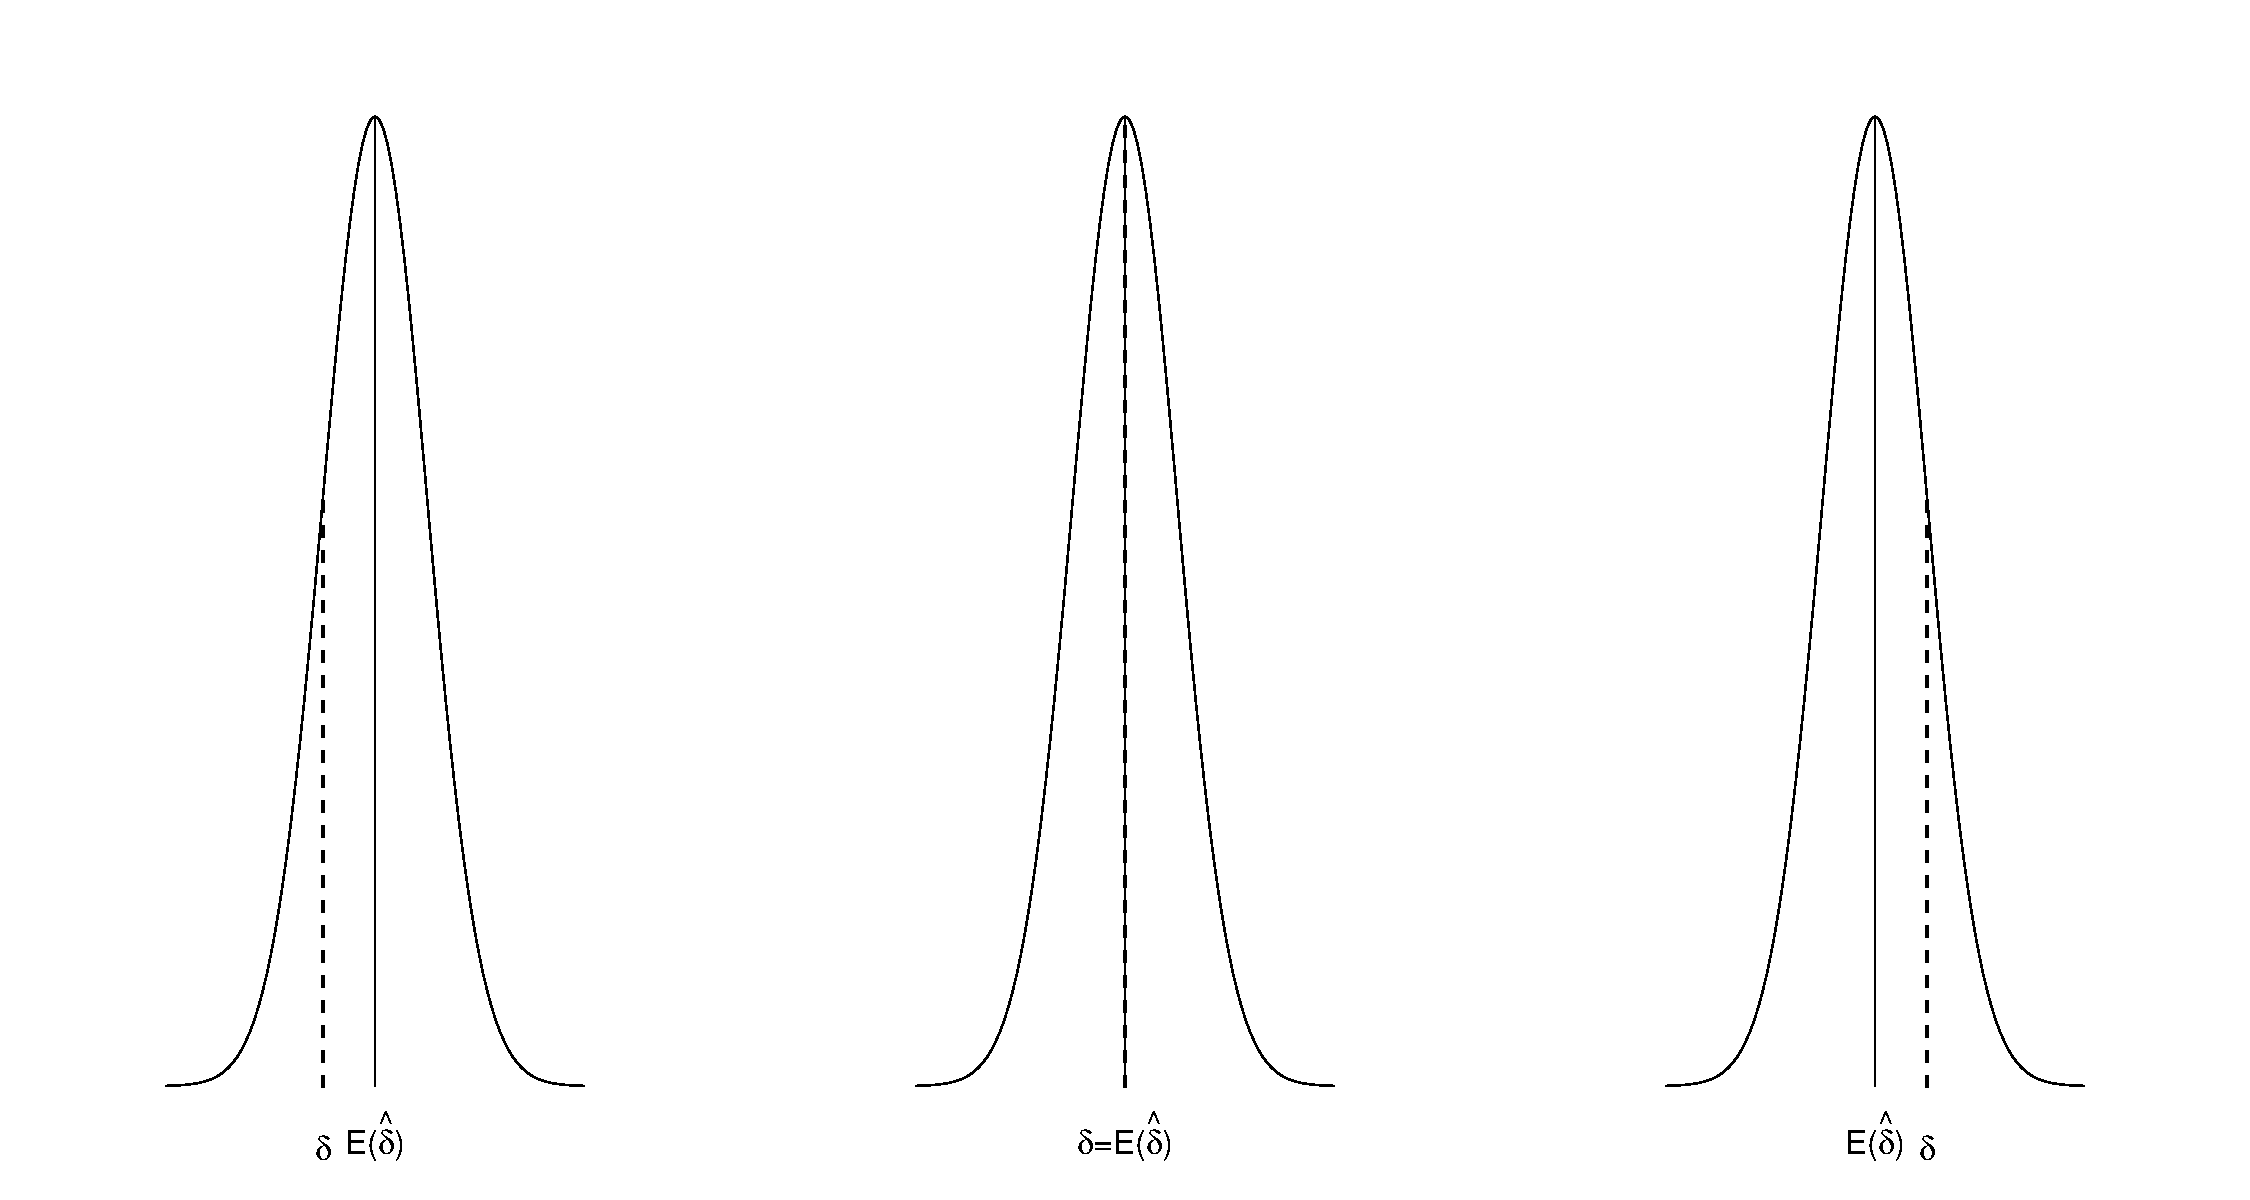
\includegraphics[width=400px]{chp4_files/figure-latex/BIAS-1} \caption{Sampling distribution for a positively biased (left), an unbiased (center) and a negatively biased estimator (right)}\label{fig:BIAS}
\end{figure}

As we can see in Tables 1 and 2 the bias is directly related to the population effect size. The larger the population effect size, the larger the bias. It is therefore also interesting to examine the \emph{relative bias}, defined as the ratio between the bias and the population effect size :
\begin{equation} 
\delta_{relative \; bias}=\frac{E(\hat{\delta})-\delta}{\delta}
\label{eqn:RELBIAS}
\end{equation}
While the bias informs us about the quality of estimates on average, in particular their capacity of lying close to the true value, it says nothing about individual estimates. Imagine a situation where the distribution of estimates is centered around the real parameter but with such a large variance that some point estimates are very far from the center. This would be problematic, since any single estimate might be very far from the true population value. Therefore it is not only essential for an estimator to be unbiased, but it is also desirable that the variability of its sampling distribution is small. Ideally, sample estimates are close to the true population parameter. Among two unbiased estimators \(\hat{\delta_1}\) and \(\hat{\delta_2}\), we therefore say that \(\hat{\delta_1}\) is \emph{more efficient} than \(\hat{\delta_2}\) if
\begin{equation} 
Var(\hat{\delta}_1) \leq Var(\hat{\delta}_2)
\label{eqn:EFFICIENCY}
\end{equation}
where \(Var(\hat{\delta})\) is the variance of the sampling distribution of the estimator \(\hat{\delta}\). Among all unbiased estimators, the more efficient estimator will be the one with the smallest variance.\footnote{The Cramér-Rao inequality provides a theoretical lower bound for the variance of unbiased estimators. An estimator reaching this bound is therefore optimally efficient.} The variance of an estimator \(\hat{\delta}\) is a function of its size (the larger the estimator, the larger the variance) and, therefore, we might be interested in evaluating the \emph{relative variance} as the ratio between the variance and the square of the population estimator :
\begin{equation} 
relative \; var(\hat{\delta}_1)=\frac{Var(\hat{\delta})}{\delta^2}
\label{eqn:RELVAR}
\end{equation}
Note that both unbiasedness and efficiency are very important when choosing an estimator. In some situations, it might be better to have a slightly biased estimator with low variance, (so that each estimate remains relatively close to the true parameter and one might be able to apply bias correction techniques) rather than an unbiased estimator with a large variance (\textbf{raviv\_bias\_2014?}).

Finally, the last property of a good point estimator is \emph{consistency}. Consistency means that the bigger the sample size, the closer the estimate is to the population parameter. In other words, the estimates \emph{converge} to the true population parameter.

\hypertarget{different-measures-of-effect-sizes}{%
\subsection{Different measures of effect sizes}\label{different-measures-of-effect-sizes}}

The \emph{d}-family effect sizes are commonly used for mean differences between groups or conditions. The population effect size is defined as
\begin{equation} 
\delta = \frac{\mu_{1}-\mu_{2}}{\sigma} 
\label{eqn:Cohendelta}
\end{equation}
where both populations follow a normal distribution with mean \(\mu_j\) in the \(j^{th}\) population (\(j=1,2\)) and standard deviation \(\sigma\). There exist different estimators of this effect size measure. For all, the mean difference is estimated by the difference \(\bar{X}_1-\bar{X}_2\) of both sample means. When the equality of variances assumption is assumed, \(\sigma\) is estimated by pooling both sample standard deviations (\(S_1\) and \(S_2\)). When the equality of variances assumption cannot be assumed, alternatives to the pooled standard deviation are available. In the next section we will present effect sizes that assume equal variances between groups (Cohen's \(d\) and Hedges' \(g\)), and effect sizes that do not assume equal variances (Glass's \(d\), Shieh's \(d\), Cohen's \(d^*\), Glass's \(g\), Shieh's \(g\), and Hedges' \(g^*\)). For each effect size we will provide information about their theoretical bias, variance, and consistency.

\hypertarget{when-variances-are-equal-between-groups}{%
\subsubsection{When variances are equal between groups}\label{when-variances-are-equal-between-groups}}

When we have good reasons to assume equality of variances between groups then the most common estimator of \(\delta\) is Cohen's \(d\), where the sample mean difference is divided by a pooled error term (\textbf{cohen\_statistical\_1965?}) :
\begin{equation*} 
Cohen's \; d = \frac{\bar{X}_1-\bar{X}_2}{\sqrt{\frac{(n_1-1) \times S_1^2+(n_2-1) \times S_2^2}{n_1+n_2-2}}}
\label{eqn:Cohends}
\end{equation*}
where \(S_j\) is the standard deviation, and \(n_j\) the sample size of the \(j^{th}\) sample (\(j=1,2\)). The reasoning behind this measure is to make use of the fact that both samples share the same population variance (Keselman et al., 2008), which means a more accurate estimation of the population variance can be achieved by pooling both estimates of this parameter (i.e.~\(S_1\) and \(S_2\)). Since the larger the sample size, the more accurate the estimate, we give more weight to the estimate based on the larger sample size. Cohen's \(d\) is directly related to Student's \emph{t}-statistic :
\begin{equation} 
t_{Student}=\frac{Cohen's \; d}{\sqrt{\frac{1}{n_1}+\frac{1}{n_2}}}\leftrightarrow Cohen's \; d =  t_{Student} \times \sqrt{\frac{1}{n_1}+\frac{1}{n_2}}
\label{eqn:Cohenvsstudent}
\end{equation}
Under the assumption of normality and equal variances between groups, Student's \emph{t}-statistic follows a \emph{t}-distribution with known degrees of freedom
\begin{equation} 
df_{Student} = n_1+n_2-2
\label{eqn:studentdf}
\end{equation}
and noncentrality parameter\footnote{Under the null hypothesis of no differences between sample means, Student's $t$-statistic will follow a central $t$-distribution with $n_1+n_2-2$ degrees of freedom. However, when the null hypothesis is false, the distribution of this quantity will not be centered, and a noncentral $t$-distribution will arise.}
\[ncp_{Student} = \frac{\delta_{Cohen}}{\sqrt{\frac{1}{n_1}+\frac{1}{n_2}}}\]
where \(\delta_{Cohen}= \frac{\mu_1-\mu_2}{\sigma_{pooled}}\) and \(\sigma_{pooled}= \sqrt{\frac{(n_1-1) \times \sigma^2_1+(n_2-1) \times \sigma^2_2}{n_1+n_2-2}}\). The relationship described in equation \ref{eqn:Cohenvsstudent} and the theoretical distribution of Student's \emph{t}-statistic allow us to determine the sampling distribution of Cohen's \(d\), and therefore, its expectation and variance when the assumptions of normality and equal variances are met. All these equations are provided in Table 1. For interested readers, Supplemental Material 1 provides a detailed examination of the theoretical bias and variance of Cohen's \(d\) based on Table 1, as well as the bias and variance of all other estimators described later, based on Tables 2 and 3, with the goal to determine which parameters influence the bias and variance of different estimators. The main results will be discussed in the section ``Monte Carlo Simulations : assessing the bias, efficiency and consistency of 5 estimators'' below.

While Cohen's \(d\) is a consistent estimator, its bias and variance are substantial with small sample sizes, even under the assumptions of normality and equal variances (\textbf{lakens\_calculating\_2013?}). In order to compensate for Cohen's \(d\) bias with small sample sizes, Hedges and Olkin (1985) defined a bias-corrected version :
\begin{equation*} 
Hedges' \; g = Cohen's \; d \times \frac{\Gamma(\frac{df_{Student}}{2})}{\sqrt{\frac{df_{Student}}{2}} \times \Gamma(\frac{df_{Student}-1}{2})}
\label{eqn:Hedgesgs}
\end{equation*}
where \(df_{Student}\) has been defined in equation \ref{eqn:studentdf} and \(\Gamma()\) is the gamma function (for integers, \(\Gamma(x)\) is the factorial of \(x\) minus \(1\) : \(\Gamma(x)=(x-1)!\); Goulet-Pelletier \(\&\) Cousineau, 2018). This equation can be approximated as follows :
\begin{equation*} 
Hedges' \; g = Cohen's \; d \times \left( 1- \frac{3}{4N -9} \right)
\label{eqn:Hedgesgsapprox}
\end{equation*}
where \(N\) is the total sample size. Hedges' \(g\) is theoretically unbiased when the assumptions of normality and equal variances are met (see Table 1). Moreover, while the variance of both Cohen's \(d\) and Hedges' \(g\) depend on the same parameters (i.e.~the total sample size (\(N\)) and the sample sizes ratio \(\left(\frac{n_2}{n_1}\right)\)), Hedges' \(g\) is less variable, especially with small sample sizes.\footnote{In Table 1, one can see that the variance of Hedges' $g$ equals the variance of Cohen's $d$, multiplied by $\left[\frac{\Gamma(\frac{df}{2})}{\sqrt{\frac{df}{2}} \times \Gamma(\frac{df-1}{2})} \right] ^2$. This term is always less than 1 and tends to 1 when the sample sizes tends to infinity ($52 \le \left[\frac{\Gamma(\frac{df}{2})}{\sqrt{\frac{df}{2}} \times \Gamma(\frac{df-1}{2})} \right] ^2 < 1$ for $3 \le df < \infty$). As a consequence, the larger the total sample size, the smaller the difference between the variance of Cohen's $d$ and Hedges' $g$.}

While the pooled error term is the best choice when variances are equal between groups (\textbf{grissom\_review\_2001?}), it may not be well advised for use with data that violate this assumption (Cumming, 2013; Grissom \& Kim, 2001; Grissom \& Kim, 2005; Kelley, 2005; Shieh, 2013). When variances are unequal between groups, the expression in equation 5 is no longer valid because both groups do not share a common population variance. If we pool the estimates of two unequal population variances, the estimator of effect size will be smaller as it should be in case of positive pairing (i.e.~the group with the larger sample size is extracted from the population with the larger variance) and larger as it should be in case of negative pairing (i.e.~the group with the larger sample size is extracted from the population with the smaller variance). Because the assumption of equal variances across populations is rarely realistic in practice (Cain et al., 2017; Delacre et al., 2017; Delacre et al., 2019; Erceg-Hurn \& Mirosevich, 2008; Glass et al., 1972; Grissom, 2000; Micceri, 1989; Yuan et al., 2004), both Cohen's \(d\) and Hedges' \(g\) should be abandoned in favor of an alternative robust to unequal population variances.

\newpage
\begin{landscape}

\begin{longtable}[]{@{}
  >{\raggedright\arraybackslash}p{(\columnwidth - 6\tabcolsep) * \real{0.13}}
  >{\centering\arraybackslash}p{(\columnwidth - 6\tabcolsep) * \real{0.12}}
  >{\centering\arraybackslash}p{(\columnwidth - 6\tabcolsep) * \real{0.27}}
  >{\centering\arraybackslash}p{(\columnwidth - 6\tabcolsep) * \real{0.48}}@{}}
\caption{Expentency, bias and variance of Cohen's \(d_s\) and Hedges' \(g_s\) under the assumptions that independent residuals are normally distributed with equal variances across groups.}\tabularnewline
\toprule
\begin{minipage}[b]{\linewidth}\raggedright
\end{minipage} & \begin{minipage}[b]{\linewidth}\centering
df
\end{minipage} & \begin{minipage}[b]{\linewidth}\centering
Expectation
\end{minipage} & \begin{minipage}[b]{\linewidth}\centering
Variance
\end{minipage} \\
\midrule
\endfirsthead
\toprule
\begin{minipage}[b]{\linewidth}\raggedright
\end{minipage} & \begin{minipage}[b]{\linewidth}\centering
df
\end{minipage} & \begin{minipage}[b]{\linewidth}\centering
Expectation
\end{minipage} & \begin{minipage}[b]{\linewidth}\centering
Variance
\end{minipage} \\
\midrule
\endhead
Cohen's \(d_s\) & \(N-2\) & \(\delta_{Cohen} \times c_f\) & \(\frac{N\times df}{n_1n_2 \times (df-2)} + \delta^2_{Cohen} \left[ \frac{df}{df-2} - c_f^2\right]\) \\
& & & \\
& & \(\approx \frac{\delta_{Cohen}}{\left(1-\frac{3}{4N-9}\right)}\) & \(\approx \frac{N\times df}{n_1n_2 \times (df-2)} + \delta^2_{Cohen} \left[ \frac{df}{df-2} - \left( \frac{1}{1-\frac{3}{4N-9} }\right)^2\right]\) \\
& & & \\
& & & \\
Hedges' \(g_s\) & \(N-2\) & \(\delta_{Cohen}\) & \(Var(Cohen's \; d_s) \times \left[ \frac{\Gamma(\frac{df}{2})}{\sqrt{\frac{df}{2}} \times \Gamma(\frac{df-1}{2})} \right]^2\) \\
& & & \\
& & & \(\approx Var(Cohen's \; d_s) \times \left[1-\frac{3}{4N-9}\right]^2\) \\
& & & \\
\bottomrule
\end{longtable}

\emph{Note}. \(\delta_{Cohen}= \frac{\mu_1-\mu_2}{\sigma_{pooled}}\) and \(c_f=\frac{\sqrt{\frac{df}{2}} \times \Gamma\left( \frac{df-1}{2}\right)}{\Gamma\left( \frac{df}{2}\right)}\); Cohen's \(d_s\) is a biased estimator, because its expectation differs from the population effect size. Moreover, the larger the population estimator (\(\delta_{Cohen}\)), the larger the bias. Indeed, the bias is the difference between the expectation and \(\delta_{Cohen}\): \(\delta_{bias} = \delta_{Cohen} \times (c_f-1)\). On the other hand, Hedges' \(g_s\) is an unbiased estimator, because its expectation equals \(\delta_{Cohen}\); equations in Table 1 require \(df \ge 3\) (i.e.~\(N \ge 5\)).

\end{landscape}

\hypertarget{when-variances-are-unequal-between-populations}{%
\subsubsection{When variances are unequal between populations}\label{when-variances-are-unequal-between-populations}}

In his review, (\textbf{shieh\_confidence\_2013?}) mentions three options available in the literature to deal with the case of unequal variances : (A) the Glass's \(d\), (B) the Shieh's \(d\) and (C) the Cohen's \(d^*\).

\hypertarget{glasss-bmd}{%
\paragraph{\texorpdfstring{Glass's \(\bm{d}\)}{Glass's \textbackslash bm\{d\}}}\label{glasss-bmd}}

When comparing one control group with one experimental group, Glass et al.~(1981) recommend using the standard deviation of the control group as standardizer. This yields
\begin{equation*} 
Glass's \; d = \frac{\bar{X}_{e} - \bar{X}_{c}}{S_{c}}
\label{eqn:Glassds}
\end{equation*}
where \(\bar{X}_{e} \; and \; \bar{X}_{c}\) are the sample means of the experimental and control groups, and \(S_{c}\) is the sample SD of the control group. One argument in favour of using \(S_c\) as standardizer is the fact that it is not affected by the experimental treatment. When it is easy to identify which group is the ``control'' one, it is therefore convenient to compare the effect size estimation of different designs studying the same effect (\textbf{cumming\_cohens\_2013?}). However, defining this group is not always obvious (\textbf{coe\_its\_2002?}). This could induce large ambiguity because depending on the chosen \(SD\) as standardizer, measures could be substantially different (\textbf{shieh\_confidence\_2013?}). The distribution of Glass's \(d\) is defined as in Algina et al.~(2006) :
\begin{equation} 
Glass's \; d \sim \sqrt{\frac{1}{n_{c}}+\frac{\sigma_{e}^2}{n_{e} \times \sigma^2_{c}}} \times t_{df,ncp}
\label{eqn:glassvst}
\end{equation}
where \(n_c\) and \(n_e\) are the sample sizes of the control and experimental groups, and \(df\) and \(ncp\) are defined as follows :
\begin{equation} 
df = n_{c}-1
\label{eqn:glassdf}
\end{equation}
\begin{equation*} 
ncp = \frac{\delta_{Glass}}{\sqrt{\frac{1}{n_{c}} + \frac{\sigma_{e}^2}{n_{e} \times \sigma^2_{c}}}}
\label{eqn:glassncp}
\end{equation*}
where \(\delta_{Glass} = \frac{\mu_{c}-\mu_{e}}{\sigma_{c}}\) and \(\mu_c\) and \(\mu_e\) are respectively the mean of the populations control and experimental groups are extracted from. Thanks to equation \ref{eqn:glassvst}, we can compute its theoretical expectation and variance when the assumption of normality is met (see Table 2), and therefore determine which factors influence bias and variance, and how they do so (see Supplemental Material 1).

\newpage
\begin{landscape}

\begin{longtable}[]{@{}
  >{\raggedright\arraybackslash}p{(\columnwidth - 6\tabcolsep) * \real{0.11}}
  >{\centering\arraybackslash}p{(\columnwidth - 6\tabcolsep) * \real{0.20}}
  >{\centering\arraybackslash}p{(\columnwidth - 6\tabcolsep) * \real{0.18}}
  >{\centering\arraybackslash}p{(\columnwidth - 6\tabcolsep) * \real{0.51}}@{}}
\caption{Expentency, bias and variance of Glass's \(d_s\) and Cohen's \(d^*_s\) and Shieh's \(d_s\) under the assumption that independent residuals are normally distributed.}\tabularnewline
\toprule
\begin{minipage}[b]{\linewidth}\raggedright
\end{minipage} & \begin{minipage}[b]{\linewidth}\centering
df
\end{minipage} & \begin{minipage}[b]{\linewidth}\centering
Expectation
\end{minipage} & \begin{minipage}[b]{\linewidth}\centering
Variance
\end{minipage} \\
\midrule
\endfirsthead
\toprule
\begin{minipage}[b]{\linewidth}\raggedright
\end{minipage} & \begin{minipage}[b]{\linewidth}\centering
df
\end{minipage} & \begin{minipage}[b]{\linewidth}\centering
Expectation
\end{minipage} & \begin{minipage}[b]{\linewidth}\centering
Variance
\end{minipage} \\
\midrule
\endhead
Glass's \(d_s\) & \(n_c-1\) & ~\(\delta_{Glass} \times c_f\) & \(\frac{df}{df-2} \times \left( \frac{1}{n_c} + \frac{\sigma^2_e}{n_e\sigma^2_c}\right) + \delta^2_{Glass} \left( \frac{df}{df-2} - c_f^2 \right)\) \\
& & & \\
Cohen's \(d^*_s\) & \(\frac{(n_1-1)(n_2-1)(\sigma^2_1+\sigma^2_2)^2}{(n_2-1)\sigma^4_1+(n_1-1)\sigma^4_2}\) & \(\delta^*_{Cohen} \times c_f\) & \(\frac{df}{df-2} \times \frac{2\left( \frac{\sigma^2_1}{n_1} + \frac{\sigma^2_2}{n_2} \right)}{\sigma^2_1+\sigma^2_2} + (\delta^*_{Cohen})^2 \left( \frac{df}{df-2} - c_f^2 \right)\) \\
& & & \\
& & \(\approx \delta^*_{Cohen} \times \frac{4df-1}{4(df-1)}\) & \(\approx \frac{df}{df-2} \times \frac{2\left( \frac{\sigma^2_1}{n_1} + \frac{\sigma^2_2}{n_2} \right)}{\sigma^2_1+\sigma^2_2} + (\delta^*_{Cohen})^2 \left[ \frac{df}{df-2} - \left( \frac{4 \;df-1}{4(df-1)}\right)^2 \right]\) \\
& & & \\
Shieh's \(d_s\) & \(\frac{\left(\frac{\sigma^2_1}{n_1}+\frac{\sigma^2_2}{n_2} \right)^2}{\frac{(\sigma^2_1/n_1)^2}{n_1-1}+\frac{(\sigma^2_2/n_2)^2}{n_2-1}}\) & \(\delta_{Shieh} \times c_f\) & \(\frac{df}{(df-2)N} + \delta^2_{Shieh} \left( \frac{df}{df-2} - c_f^2 \right)\) \\
& & & \\
\bottomrule
\end{longtable}

\emph{Note}. \(c_f=\frac{\sqrt{\frac{df}{2}} \times \Gamma\left( \frac{df-1}{2}\right)}{\Gamma\left( \frac{df}{2}\right)}\); \(\delta_{Glass}=\frac{\mu_c-\mu_e}{\sigma_c}\), \(\delta_{Shieh}=\frac{\mu_1-\mu_2}{\sqrt{\frac{\sigma^2_1}{n_1/N}+\frac{\sigma^2_2}{n_2/N}}}\) and \(\delta^*_{Cohen}=\frac{\mu_1-\mu_2}{\sqrt{\frac{\sigma^2_1+\sigma^2_2}{2}}}\); all estimators are biased estimators, because their expectations differ from the population effect size \(\delta\). Moreover, the larger the population estimator (\(\delta\)), the larger the bias. Indeed, the bias is the difference between the expectation and \(\delta\): \(\delta_{bias} = \delta \times (c_f-1)\); equations in Table 2 require \(df \ge 3\) and at least 2 subjects per group.

\end{landscape}
\newpage

\hypertarget{shiehs-bmd}{%
\paragraph{\texorpdfstring{Shieh's \(\bm{d}\)}{Shieh's \textbackslash bm\{d\}}}\label{shiehs-bmd}}

Kulinskaya and Staudte (2007) were the first to recommend the use of a standardizer that takes the sample sizes allocation ratios into account, in addition to the variance of both samples. (\textbf{shieh\_confidence\_2013?}), following Kulinskaya and Staudte, proposed a modification of the exact \emph{SD} of the sample mean difference :
\begin{equation*} 
Shieh's \; d = \frac{\bar{X}_1 - \bar{X}_2}{\sqrt{S_1^2/q_1+S_2^2/q_2}}; \;\;\; q_j=\frac{n_j}{N} (j=1,2)
\label{eqn:Shiehds}
\end{equation*}
where \(N = n_1+n_2\). Shieh's \(d\) is directly related with Welch's \emph{t}-statistic :
\begin{equation} 
Shieh's \; d=\frac{t_{Welch}}{\sqrt{N}}\leftrightarrow t_{welch} = Shieh's \; d \times \sqrt{N}
\label{eqn:shiehvswelch}
\end{equation}
The exact distribution of Welch's \emph{t}-statistic is more complicated than the exact distribution of Student's \emph{t}-statistic, but it can be approximated, under the assumption of normality, by a \emph{t}-distribution with degrees of freedom and noncentrality parameters (\textbf{welch\_significance\_1938?}) :
\begin{equation} 
df_{Welch} = \frac{\left(\frac{\sigma^2_1}{n_1}+\frac{\sigma^2_2}{n_2} \right)^2}{\frac{(\sigma^2_1/n_1)^2}{n_1-1}+\frac{(\sigma^2_2/n_2)^2}{n_2-1}}
\label{eqn:welchdf}
\end{equation}
\begin{equation*} 
ncp_{Welch} = \delta_{Shieh} \times \sqrt{N} = \frac{\mu_1-\mu_2}{\sqrt{\frac{\sigma_1^2}{n1}+\frac{\sigma_2^2}{n_2}}}
\label{eqn:welchncp}
\end{equation*}
where \(\delta_{Shieh}=\frac{\mu_1-\mu_2}{\sqrt{\frac{\sigma_1^2}{n_1/N}+\frac{\sigma_2^2}{n_2/N}}}\). The relationship described in equation \ref{eqn:shiehvswelch} and the theoretical distribution of Welch's \emph{t}-statistic allow us to approximate the sampling distribution of Shieh's \(d\). Based on the sampling distribution of Shieh's \(d\), we can estimate its theoretical expectation and variance under the assumption of normality (see Table 2), and thereby determine which factors influence bias and variance, and how they do so (see Supplemental Material 1).

As demonstrated in the Appendix, when variances and sample sizes are equal across groups, the biases and variances of Cohen's \(d\) and Shieh's \(d\) are identical except for multiplication by a constant. The same is true for the estimators \(\delta_{Cohen}\) and \(\delta_{Shieh}\) :\\
\begin{equation} 
\delta_{Cohen} = 2 \times \delta_{Shieh} \quad (\mbox{considering} \; \sigma_1 = \sigma_2 \; \mbox{and} \; n_1 = n_2)
\label{eqn:CohenShieh}
\end{equation}
\begin{equation} 
Bias_{Cohen's \; d} = 2 \times Bias_{Shieh's \; d} \quad (\mbox{considering} \; \sigma_1 = \sigma_2 \; \mbox{and} \; n_1 = n_2)
\label{eqn:biasCohenshieh}
\end{equation}
\begin{equation} 
Var_{Cohen's \; d} = 4 \times Var_{Shieh's \; d} \quad (\mbox{considering}\; \sigma_1 = \sigma_2 \; \mbox{and} \; n_1 = n_2)
\label{eqn:varCohenshieh}
\end{equation}
We can deduce from equations \ref{eqn:CohenShieh}, \ref{eqn:biasCohenshieh} and \ref{eqn:varCohenshieh} that relative to their respective population effect size, Cohen's \(d\) and Shieh's \(d\) are equally accurate. In other words, their relative bias and variance are identical. This is a good illustration of our motivation to favor relative bias and variance (previously defined in equations \ref{eqn:RELBIAS} and \ref{eqn:RELVAR}) over the most commonly used raw bias and variance (previously defined in equations \ref{eqn:BIAS} and \ref{eqn:EFFICIENCY}).

When sample sizes are not equal, according to the statistical properties of Welch's statistic under heteroscedasticity, Shieh's \(d\) accounts for the allocation ratio of sample sizes to each condition. The lack of generality caused by taking this specificity of the design into account has led (\textbf{cumming\_cohens\_2013?}) to question its usefulness in terms of interpretability : when the mean difference (\(\bar{X_1}-\bar{X_2}\)), \(S_1\), and \(S_2\) remain constant, Shieh's \(d\) will vary as a function of the sample sizes allocation ratio (unlike Cohen's \(d^*\) that we will define below). At the population level, \(\delta_{Shieh}\) also depends on the sample sizes allocation ratio, as illustrated in the following shiny application : \url{https://effectsize.shinyapps.io/ShiehvsCohen/}.

\hypertarget{cohens-bmd}{%
\paragraph{\texorpdfstring{Cohen's \(\bm{d^*}\)}{Cohen's \textbackslash bm\{d\^{}*\}}}\label{cohens-bmd}}

An effect size estimator based on the sample mean difference divided by the square root of the non pooled average of both variance estimates was suggested by (\textbf{welch\_significance\_1938?}). Here, we indicate the difference between Cohen's \(d\) (based on the pooled standard deviations) and Cohen's \(d^*\) with an asterisk. This yields :
\begin{equation*} 
Cohen's \; d^* = \frac{\bar{X}_{1} - \bar{X}_{2}}{ \sqrt{\frac{\left(S^2_{1}+S^2_{2} \right)}{2}}}
\label{eqn:Cohenprimeds}
\end{equation*}
where \(\bar{X}_{j}\) is the mean and \(S_j\) is the standard deviation of the \(j^{th}\) sample (j = 1,2). We know the distribution of Cohen's \(d^*\) (\textbf{huynh\_unified\_1989?}) :
\begin{equation} 
Cohen's \; d^* \sim  \sqrt{\frac{2(n_2\times\sigma^2_1+n_1\times\sigma^2_2)}{n_1n_2(\sigma^2_1+\sigma^2_2)}} \times t_{df^*,ncp^*}
\label{eqn:Cohendprimedist}
\end{equation}
Where \(df^*\) and \(ncp^*\) are defined as follows :
\begin{equation} 
df^* = \frac{(n_1-1)(n_2-1)(\sigma^2_1+\sigma^2_2)^2}{(n_2-1)\sigma^4_1+(n_1-1)\sigma^4_2}
\label{eqn:Cohendprimedf}
\end{equation}
\begin{equation*} 
ncp^*=\delta^*_{Cohen} \times \sqrt{\frac{n_1n_2(\sigma^2_1+\sigma^2_2)}{2(n_2\sigma^2_1+n_1\sigma^2_2)}}=\frac{\mu_1-\mu_2}{\sqrt{\frac{\sigma_1^2}{n_1}+\frac{\sigma^2_2}{n_2}}}
\label{eqn:Cohendprimevst}
\end{equation*}
where \(\delta^*_{Cohen}=\frac{\mu_1-\mu_2}{\sqrt{\frac{\sigma^2_1+\sigma^2_2}{2}}}\). Using equation \ref{eqn:Cohendprimedist} we can compute its theoretical expectation and variance when the assumption of normality is met (see Table 2), and therefore determine which factors influence bias and variance, and how they do so (see Supplemental Material 1). This estimator has been widely criticized, because it results in a variance term of an artificial population (i.e.~since the variance term does not estimate the variance of one or the other group, the composite variance is an estimation of the variance of an artificial population; Grissom \(\&\) Kim, 2001), and unless both sample sizes are equal, the variance term does not correspond to the variance of the mean difference (\textbf{shieh\_confidence\_2013?}). However, we will show throughout the simulation section that this estimator exhibits very good inferential properties. Moreover, it has a constant value across sample sizes ratios, as shown in the Shiny App at \url{https://effectsize.shinyapps.io/ShiehvsCohen/}.

\hypertarget{glasss-bmg-shiehs-bmg-and-hedges-bmg}{%
\paragraph{\texorpdfstring{Glass's \(\bm{g}\), Shieh's \(\bm{g}\) and Hedges' \(\bm{g^*}\)}{Glass's \textbackslash bm\{g\}, Shieh's \textbackslash bm\{g\} and Hedges' \textbackslash bm\{g\^{}*\}}}\label{glasss-bmg-shiehs-bmg-and-hedges-bmg}}

As for Cohen's \(d\), a Hedges' correction can be applied in order to compensate for the bias of Glass's \(d\), Shieh's \(d\) and Cohen's \(d^*\) with small sample sizes (see Table 2). This correction has the following general form :
\begin{equation*} 
g = d \times \frac{\Gamma(\frac{\nu}{2})}{\sqrt{\frac{\nu}{2}} \times \Gamma(\frac{\nu-1}{2})}
\end{equation*}
where the distinct values of \(\nu\) are provided in equation \ref{eqn:glassdf} for Glass's \(g\), in equation \ref{eqn:welchdf} for Shieh's \(g\) and in equation and \ref{eqn:Cohendprimedf} for Hedges' \(g^*\). The three corrected estimators are theoretically unbiased when the assumption of normality is met. Their variance is a function of the same parameters as their biased equivalent. However, due to the correction they have a smaller variance, especially with small sample sizes, as shown in Table 3. In summary :

\begin{itemize}
\tightlist
\item
  The variances of Hedges' \(g^*\) and Shieh's \(g\) depend on the total sample size (\(N\)), their respective population effect size (\(\delta\)), and the interaction between the sample sizes ratio and the \(SD\)-ratio \(\left(\frac{n_2}{n_1}\times\frac{\sigma_2}{\sigma_1} \right)\).\\
\item
  The variance of Glass's \(g\) also depends on \(N\), \(\delta\) and \(\frac{n_c}{n_e}\times\frac{\sigma_c}{\sigma_e}\). In addition, there is also a main effect of the \(SD\)-ratio \(\left(\frac{\sigma_c}{\sigma_e} \right)\) on its variance.
\end{itemize}

How these parameters influence the variance of the estimators will be summarized and illustrated in Monte Carlo simulations below.

\newpage
\begin{landscape}

\begin{longtable}[]{@{}
  >{\raggedright\arraybackslash}p{(\columnwidth - 6\tabcolsep) * \real{0.11}}
  >{\centering\arraybackslash}p{(\columnwidth - 6\tabcolsep) * \real{0.20}}
  >{\centering\arraybackslash}p{(\columnwidth - 6\tabcolsep) * \real{0.18}}
  >{\centering\arraybackslash}p{(\columnwidth - 6\tabcolsep) * \real{0.51}}@{}}
\caption{Expectation, bias and variance of Glass's \(d_s\) and Cohen's \(d^*_s\) and Shieh's \(d_s\) under the assumption that independent residuals are normally distributed.}\tabularnewline
\toprule
\begin{minipage}[b]{\linewidth}\raggedright
\end{minipage} & \begin{minipage}[b]{\linewidth}\centering
df
\end{minipage} & \begin{minipage}[b]{\linewidth}\centering
Expectation
\end{minipage} & \begin{minipage}[b]{\linewidth}\centering
Variance
\end{minipage} \\
\midrule
\endfirsthead
\toprule
\begin{minipage}[b]{\linewidth}\raggedright
\end{minipage} & \begin{minipage}[b]{\linewidth}\centering
df
\end{minipage} & \begin{minipage}[b]{\linewidth}\centering
Expectation
\end{minipage} & \begin{minipage}[b]{\linewidth}\centering
Variance
\end{minipage} \\
\midrule
\endhead
Glass's \(g_s\) & \(n_c-1\) & ~\(\delta_{glass}\) & \(Var(Glass's \; d_s) \times \left( \frac{\Gamma\left(\frac{df}{2} \right)}{\sqrt{\frac{df}{2}} \times \Gamma \left( \frac{df-1}{2}\right)}\right)^2\) \\
& & & \\
Cohen's \(g^*_s\) & \(\frac{(n_1-1)(n_2-1)(\sigma^2_1+\sigma^2_2)^2}{(n_2-1)\sigma^4_1+(n_1-1)\sigma^4_2}\) & \(\delta^*_{Cohen}\) & \(Var(Cohen's \; d^*_s) \times \left( \frac{\Gamma\left(\frac{df}{2} \right)}{\sqrt{\frac{df}{2}} \times \Gamma \left( \frac{df-1}{2}\right)}\right)^2\) \\
& & & \\
Shieh's \(g_s\) & \(\approx \frac{\left(\frac{\sigma^2_1}{n_1}+\frac{\sigma^2_2}{n_2} \right)^2}{\frac{(\sigma^2_1/n_1)^2}{n_1-1}+\frac{(\sigma^2_2/n_2)^2}{n_2-1}}\) & \(\delta_{Shieh}\) & \(Var(Shieh's \; d_s) \times \left( \frac{\Gamma\left(\frac{df}{2} \right)}{\sqrt{\frac{df}{2}} \times \Gamma \left( \frac{df-1}{2}\right)}\right)^2\) \\
& & & \\
\bottomrule
\end{longtable}

\emph{Note}. \(c_f=\frac{\sqrt{\frac{df}{2}} \times \Gamma\left( \frac{df-1}{2}\right)}{\Gamma\left( \frac{df}{2}\right)}\); \(\delta_{Glass}=\frac{\mu_c-\mu_e}{\sigma_c}\), \(\delta_{Shieh}=\frac{\mu_1-\mu_2}{\sqrt{\frac{\sigma^2_1}{n_1/N}+\frac{\sigma^2_2}{n_2/N}}}\) and \(\delta^*_{Cohen}=\frac{\mu_1-\mu_2}{\sqrt{\frac{\sigma^2_1+\sigma^2_2}{2}}}\); all estimators are unbiased estimators, because their expectations equal the population effect size \(\delta\); equations in Table 3 require \(df \ge 3\) and at least 2 subjects per group.

\end{landscape}
\newpage

\hypertarget{monte-carlo-simulations}{%
\subsubsection{Monte Carlo Simulations}\label{monte-carlo-simulations}}

\hypertarget{assessing-the-bias-efficiency-and-consistency-of-5-estimators}{%
\paragraph{Assessing the bias, efficiency and consistency of 5 estimators}\label{assessing-the-bias-efficiency-and-consistency-of-5-estimators}}

\hypertarget{method}{%
\subparagraph{Method}\label{method}}

We performed Monte Carlo simulations using R (version 3.5.0) to assess the bias, efficiency and consistency of Hedges \(g\), Glass's \(g\) (using respectively the sample \(SD\) of the first or second group as a standardizer), Hedges' \(g^*\) and Shieh's \(g\).

A set of 100,000 datasets was generated for 1,008 scenarios as a function of different criteria. In 252 scenarios, samples were extracted from a normally distributed population (in order to ensure the reliability of our calculation method) and in 756 scenarios, samples were extracted from non normal population distributions. In order to assess the quality of estimators under realistic deviations from the normality assumption, we referred to the review of Cain et al.~(2017). Cain et al.~(2017) investigated 1,567 univariate distributions from 194 studies published by authors in Psychological Science (from January 2013 to June 2014) and the American Education Research Journal (from January 2010 to June 2014). For each distribution, they computed Fisher's skewness
\[G_{1}=\frac{\sqrt{n(n-1)}}{n-2} \frac{m_{3}}{\sqrt{(m_{2})^3}}\]
and kurtosis \[G_{2}=\frac{n-1}{(n-2)(n-3)}\times \left[(n+1)\left(\frac{m_{4}}{(m_{2})^2}-3\right)+6\right]\]
where \(n\) is the sample size and \(m_{2}\), \(m_{3}\) and \(m_{4}\) are respectively the second, third and fourth centered moments. They found values of kurtosis from \(G_2\) = -2.20 to 1,093.48. According to their suggestions, throughout our simulations, we kept constant the population kurtosis value at the 99th percentile of their distribution of kurtosis, i.e.~\(G_2\)=95.75. Regarding skewness, we simulated population parameter values which correspond to the 1st and 99th percentile of their distribution of skewness, i.e.~respectively \(G_1\) = -2.08 and \(G_1\) = 6.32. We also simulated samples extracted from population where \(G_1\) = 0, in order to assess the main effect of high kurtosis on the quality of estimators. All possible combinations of population skewness and kurtosis and the number of scenarios for each combination are summarized in Table 4.

\begin{longtable}[]{@{}ccccc@{}}
\caption{Number of combinations of skewness and kurtosis in our simulations.}\tabularnewline
\toprule
& & & \textbf{Kurtosis} & \\
\midrule
\endfirsthead
\toprule
& & & \textbf{Kurtosis} & \\
\midrule
\endhead
& & 0 & 95.75 & \textbf{TOTAL} \\
& & --------------- & -------------- & --------------- \\
& 0 & 252 & 252 & \textbf{504} \\
& & & & \\
\textbf{Skewness} & -2.08 & / & 252 & \textbf{252} \\
& & & & \\
& 6.32 & / & 252 & \textbf{252} \\
& & & & \\
& \textbf{TOTAL} & \textbf{252} & \textbf{756} & \textbf{1008} \\
\bottomrule
\end{longtable}

\emph{Note.} Fisher's skewness (G1) and kurtosis (G2) are presented in Table 4. The 252 combinations where both G1 and G2 equal 0 correspond to the normal case.

For the 4 resulting combinations of skewness and kurtosis (see Table 4), all other parameter values were chosen in order to illustrate the consequences of factors identified as playing a key role on the variance of unbiased estimators. We manipulated the population mean difference (\(\mu_1-\mu_2\)), the sample sizes (\emph{n}), the sample size ratio (\emph{n}-ratio = \(\frac{n_2}{n_1}\)), the population \emph{SD}-ratio (i.e.~\(\frac{\sigma_2}{\sigma_1}\)), and the sample size and population variance pairing \(\left(\frac{n_2}{n_1}\times\frac{\sigma_2}{\sigma_1} \right)\). In our scenarios, \(\mu_2\) was always 0 and \(\mu_1\) varied from 1 to 4, in steps of 1 (so does \(\mu_1-\mu_2\)).\footnote{In the original plan, we had added 252 simulations in which $\mu_1$ and $\mu_2$ were both null. We decided not to present the results of these simulations in the main article, because the relative bias and the relative variance appeared to us to be very useful to fully understand the comparison of the estimators, and computing them is impossible when the real mean difference is zero. Indeed, for these specific configurations, both relative bias and relative variance would have infinite values due to the presence of the population effect size term in their denominator. However, these extra simulations were included in the simulation checks, in Supplemental Material 2. } Moreover, \(\sigma_1\) always equals 1, and \(\sigma_2\) equals .1, .25, .5, 1, 2, 4 or 10, and therefore, the \(SD\)-ratio were 10, 4, 2, 1, .5, .25 or .1. The simulations for which both \(\sigma_1\) and \(\sigma_2\) equal 1 are the particular case of homoscedasticity, or equal population variances across groups. The sample sizes of both groups (\(n_1\) and \(n_2\)) were 20, 50 or 100. When sample sizes of both groups are equal, the \emph{n}-ratio equals 1 (this is known as a balanced design). All possible combinations of \emph{n}-ratio and population \emph{SD}-ratio were simulated in order to distinguish scenarios where both sample sizes and population variances are unequal across groups (with positive pairing when the group with the largest sample size is extracted from the population with the largest \emph{SD}, and negative pairing when the group with the smallest sample size is extracted from the population with the smallest \emph{SD}) and scenarios with no pairing between sample sizes and variances (sample sizes and/or population \emph{SD} are equal across all groups). In sum, the simulations grouped over different sample sizes yield 4 conditions (a, b, c and d) based on the \emph{n}-ratio, population \emph{SD}-ratio, and sample size and population variance pairing, as summarized in Table 5. We chose to divide scenarios into these 4 conditions because analyses in Supplemental Material 1 revealed main and interaction effects of sample sizes ratio and \(SD\)-ratio on the bias and variance of some estimators.

\begin{longtable}[]{@{}ccccc@{}}
\caption{4 conditions based on the \(n\)-ratio and the \(SD\)-ratio.}\tabularnewline
\toprule
& & & \textbf{\emph{n}-ratio} & \\
\midrule
\endfirsthead
\toprule
& & & \textbf{\emph{n}-ratio} & \\
\midrule
\endhead
& & \textbf{1} & \textbf{\textgreater1} & \textbf{\textless1} \\
& & ----------- & ------------ & ------------ \\
& \textbf{1} & a & b & b \\
& & & & \\
\textbf{\emph{SD}-ratio} & \textbf{\textgreater1} & c & d & d \\
& & & & \\
& \textbf{\textless1} & c & d & d \\
\bottomrule
\end{longtable}

\hypertarget{results}{%
\subparagraph{Results}\label{results}}

Before presenting the comparison of the estimators for each condition, it is useful to make some general comments.

\begin{enumerate}
\def\labelenumi{\arabic{enumi})}
\item
  We previously discussed the fact that raw bias and variances are sometimes misleading. They can give the illusion of huge differences between two estimators, even if these differences only reflect a change of unit (i.e.~different population effect sizes). To better understand this, imagine a sample of 15 people for whom we know the height (in meters) and we compute a sample variance of 0.06838. If we convert sizes to centimeters and compute the sample variance again, we find a measure of 683.8 (i.e.~\(10^4\) larger). Both measures represent the same amount of variability, but they are expressed in different units. The same issue due to a change in scales occurs when comparing the estimates of different population measures. To avoid this possible confusion, we will only present the relative bias and relative variance in all Figures (and anytime we will mention the biases and variances in the results section, we will be referring to relative bias and variance). For interested readers, illustrations of the raw bias and variance are available on Github at \url{https://github.com/mdelacre/Effect-sizes/}.
\item
  For the sake of readability, the vertical axis differs across plots.
\item
  Throughout this section, we will \emph{compare} the relative bias and variance of different estimators, but we do not present bias and variance in absolute terms. We chose very extreme (although realistic) conditions, and we know that none of the parametric measures of effect size will be robust against such extreme conditions. Our goal is therefore to study the robustness of the estimators against normality violations only in comparison with the robustness of other indicators, but not in absolute terms.
\end{enumerate}

After these general remarks, we will analyze each condition separately. In all Figures presented below, for different sub-conditions, the averaged relative bias and relative variance of five estimators are presented. When describing the Glass's \(g\) estimators, we will systematically refer to the ``control group'' as the condition the standardizer is based on (i.e.~the first group when using \(S_1\) as standardizer, the second group when using \(S_2\) as standardizer). The other condition will be referred to as the ``experimental group.''

\emph{When variances are equal across groups}

Figures \ref{fig:idHombal} and \ref{fig:idHomunbal} represent configurations where the equality of variances assumption is met. According to our expectations, one observes that the bias of all estimators is approximately zero as long as the normality assumption is met (first column in both Figures).\footnote{When looking at relative bias for all estimators, the maximum departure from zero is 0.0064 when sample sizes are equal across groups, and 0.0065 with unequal sample sizes.} However, the more the data generation process deviations from the normality assumption (i.e.~when moving from left to right in the Figures), the larger the bias in the estimators.

We will observe that Glass's \(g\) should always be avoided when the equality of variance assumption is met. Hedges' \(g\), Hedges' \(g^*\) and Shieh's \(g\) perform equally well as long as the sample size ratio is close to 1 (condition a; see Figure \ref{fig:idHombal}). However, when designs are highly unbalanced (condition b; see Figure \ref{fig:idHomunbal}), Shieh's \(g\) is not consistent anymore, while Hedges' \(g^*\) remains consistent, Hedges's \(g\) is a better estimator. For interested readers, these findings are detailed in the three paragraphs below.

\begin{landscape}
\newpage

\begin{figure}

{\centering \includegraphics[width=1\linewidth]{C:/Users/mdelacre/Documents/Github project/Effect-sizes/Scripts outputs/Quality of ES measures/Graphs/Unbiased estimators/Combined Figures_relative quality/Hom_bal} 

}

\caption{Bias and efficiency of estimators of standardized mean difference, when variances and sample sizes are equal across groups (condition a)}\label{fig:idHombal}
\end{figure}
\end{landscape}
\newpage
\begin{landscape}

\begin{figure}

{\centering \includegraphics[width=1\linewidth]{C:/Users/mdelacre/Documents/Github project/Effect-sizes/Scripts outputs/Quality of ES measures/Graphs/Unbiased estimators/Combined Figures_relative quality/Hom_unbal} 

}

\caption{Bias and efficiency of estimators of standardized mean difference, when variances are equal across groups and sample sizes are unequal (condition b)}\label{fig:idHomunbal}
\end{figure}

\end{landscape}

Figure \ref{fig:idHombal} illustrates scenarios where both population variances and sample sizes are equal across groups (condition a). One can first notice that all estimators are consistent, as their bias and variance decrease when the total sample size increases. For any departure from the normality assumption, both bias and variance of Hedges' \(g\), Shieh's \(g\) and Hedges' \(g^*\) are similar\footnote{While the bias and variance of Cohen's $d$, Cohen's $d^*$ and Shieh's $d$ are identical, the bias and variance of Hedges' $g$ are marginally different from the bias and variance of Hedges' $g^*$ and Shieh's $g$ (these last two having identical bias and variance). Indeed, because of the sampling error, differences remain between sample variances, even when population variances are equal between groups. Since the Hedges' correction applied to Cohen's $d$ does not contain the sample variances (unlike the correction applied on both other estimators), the bias and variance of Hedges' $g$ are slighly different from the bias and variance of Hedges' $g^*$ and Shieh's $g$.} and smaller than the bias and variance of Glass's \(g\) estimates using either \(S_1\) or \(S_2\) as a standardizer. Moreover, when samples are extracted from skewed distributions, Glass's \(g\) will show different bias and variance as a function of the chosen standardizer (\(S_1\) or \(S_2\)), even if both \(S_1\) and \(S_2\) are estimates of the same population variance, based on the same sample size. This is due to non-null correlations of opposite sign between the mean difference (\(\bar{X_1}-\bar{X_2}\)) and respectively \(S_1\) and \(S_2\). In Supplemental Material 3, we detailed in which situation a non-null correlation occurs between the sample mean difference (\(\bar{X_1}-\bar{X_2}\)) and the standardizer of compared estimators as well as the way this correlation impacts the bias and variance of estimators.

Figure \ref{fig:idHomunbal} illustrates scenarios where population variances are equal across groups, but sample sizes are unequal (condition b). For any departures from the normality assumptions, Hedges' \(g\) shows the smallest bias and variance. Hedges' \(g\) and Hedges' \(g^*\) are consistent estimators (i.e.~the larger the sample sizes, the lower the bias and the variance), unlike Shieh's \(g\) and Glass's \(g\). The bias of Glass's \(g\) does not depend either on the size of the experimental group or on the total sample size. The only way to decrease the bias of Glass's \(g\) is therefore to add subjects in the control group. On the other hand, the variance of Glass's \(g\) depends on both sample sizes, but not in an equivalent way : in order to reduce the variance, it is much more efficient to add subjects in the control group and when the relative size of the experimental group decreases so does the variance, even when the total sample size is decreased. Regarding Shieh's \(g\), for a given sample size ratio, the bias and variance will decrease when sample sizes increase. However, there is a large effect of the sample sizes ratio such that when the sample sizes ratio moves away from 1 by adding subjects, bias and variance might increase.\footnote{Regarding variance, in Supplemental Material 1, we mentioned that when the population effect size is zero, the larger the total sample size, the lower the variance, whether the sample sizes ratio is constant or not. We also mentioned that this is no longer true when the population effect size is not zero. In our simulations the effect size is never zero. The effect size effect is partially visible in Figure \ref{fig:idHomunbal} because we do not entirely remove the effect size effect when we divide the variance by $\delta^2$. This is due to the fact that one term, in the equation of the variance computation, does not depend on the effect size.} On the other hand, when the sample sizes ratio moves closer to 1 by adding subjects, the bias will decrease.

When samples are extracted from skewed distributions and have unequal sizes (the two last columns in Figure \ref{fig:idHomunbal}), for a constant total sample size, Glass's \(g\), Shieh's \(g\) and Hedges' \(g^*\) will show different bias and variance depending on which group is the largest one (e.g.~when distributions are right-skewed, the bias and variance of all these estimators when \(n_1\) and \(n_2\) are respectively 50 and 20 are not the same as their bias and variance when \(n_1\) and \(n_2\) are respectively 20 and 50). This is due to a non-null correlation of opposite sign between the mean difference (\(\bar{X_1}-\bar{X_2}\)) and their respective standardizers depending on which group is the largest one, as detailed in Supplemental Material 3. One observes that under these configurations, the bias and variance of Glass's \(g\) are sometimes a bit smaller and sometimes much larger than the bias and variance of Shieh's \(g\) and Cohen's \(d^*\).\footnote{Supplemental Material 3 shows that when the $\mu_1-\mu_2 >0$ (like in our simulations), all other parameters being equal, an estimator is always less biased and variable when choosing a standardizer that is positively correlated with $\bar{X_1}-\bar{X_2}$. Supplemental Material 3 also shows that the smaller $n_c$, the larger the magnitude of correlation between $S_c$ and $\bar{X_1}-\bar{X_2}$. When $cor(S_c,\bar{X_1}-\bar{X_2})$ is positive, the positive effect of increasing the magnitude of the correlation is counterbalanced by the negative effect of reducing $n_c$. On the other hand, when $cor(S_c,\bar{X_1}-\bar{X_2})$ is negative, the negative effect of increasing the magnitude of the correlation is amplified by the negative effect of decreasing $n_c$. This explains why the difference between Glass's $g$ and other estimators is larger when Glass's $g$ is the least efficient estimator.}

\emph{When variances are unequal across groups}

Figures \ref{fig:idHetbal1} to \ref{fig:idHetunbal4} represent configurations where the equality of variances assumption is not met. According to our expectations, one observes that the bias of all estimators is approximately zero as long as the normality assumption is met (first column in all Figures), and the further from the normality assumption (i.e.~when moving from left to right in Figures), the larger the bias.\footnote{When looking at the relative bias for all estimators, the maximum departure from zero is 0.0173 when sample sizes are equal across groups, and 0.0274 when both sample sizes and variances differ across groups.} It might be considered surprising that the bias of Hedges' \(g\) remains very small throughout these conditions. As discussed in the section ``Different measures of effect size,'' Hedges' \(g\) should be avoided when population variances and sample sizes are unequal across groups, because of the pooled error term. When pooling the estimates of two unequal population variances, the resulting estimator will be smaller (in case of positive pairing) or larger (in case of negative pairing) than it should be. At the same time, when pooling two unequal population variances, the population effect size will also be smaller (in case of positive pairing) or larger (in case of negative pairing) as it should be. As a consequence, the distortion cannot be seen through the difference between the expected estimator and the population effect size measure. For this reason, the bias and variance of Hedges' \(g\) will not be taken into account in the following comparisons.

We will observe that when variances are unequal across populations, Glass's \(g\) sometimes performs better, but also sometimes performs much worst than Shieh's \(g\) and Hedges' \(g^*\), both in terms of bias and variance. The performance of Glass's \(g\) highly depends on parameters that we cannot control (i.e.~a triple interaction between the \(n\)-ratio, the \(SD\)-ratio and the correlation between the standardizer and the mean difference) and for this reason, we do not recommend using it. When the sample sizes ratio is close to 1, Shieh's \(g\) and Hedges' \(g^*\) are both appropriate but the further the sample sizes ratio is from 1, the larger the bias of Shieh's \(g\) in order that in the end, the measure that we believe performs best across scenarios is Hedges' \(g^*\).

\begin{landscape}
\newpage

\begin{figure}

{\centering \includegraphics[width=1\linewidth]{C:/Users/mdelacre/Documents/Github project/Effect-sizes/Scripts outputs/Quality of ES measures/Graphs/Unbiased estimators/Combined Figures_relative quality/Het_bal_N} 

}

\caption{Bias and efficiency of estimators of standardized mean difference, when variances are unequal across groups and sample sizes are equal (condition c), as a function of sample sizes}\label{fig:idHetbal1}
\end{figure}

\end{landscape}
\newpage
\begin{landscape}

\begin{figure}

{\centering \includegraphics[width=1\linewidth]{C:/Users/mdelacre/Documents/Github project/Effect-sizes/Scripts outputs/Quality of ES measures/Graphs/Unbiased estimators/Combined Figures_relative quality/Het_bal_sd} 

}

\caption{Bias and efficiency of estimators of standardized mean difference, when variances are unequal across groups and sample sizes are equal (condition c) as a function of the $SD$-ratio (when $n_1=n_2=20$)}\label{fig:idHetbal2}
\end{figure}

\end{landscape}
\newpage

Figures \ref{fig:idHetbal1} and \ref{fig:idHetbal2} are dedicated to scenarios where population variances are unequal between groups and sample sizes are equal (condition c). In Figure \ref{fig:idHetbal1}, scenarios are subdivided as a function of the sample sizes and one can notice that all estimators are consistent, as their bias and variance decrease when the total sample size increases. In Figure \ref{fig:idHetbal2}, scenarios are subdivided as a function of the \(SD\)-ratio. Because the comparison pattern remains very similar for all sample sizes, we present only scenarios when sample sizes equal 20. One should first notice that for all estimators in Figure \ref{fig:idHetbal2}, the relative variance seems to be much larger when \(S_2>S_1\).\footnote{The difference between the variance of estimators when the second group is 10 times larger than the first group was so large that we decided to not present it, for the sake of readability of the Figures.} This information should not be taken into account because it is only an artefact of our simulation conditions combined with the way we computed the relative variance.\footnote{We previously mentioned that when dividing the variance by $\delta^2$, we do not entirely remove the effect size effect. Actually, we introduce $\delta^2$ in the denominator of the first term, in the equation of the variance computation. Because we performed our simulations in order that $\sigma_1$ always equals 1, the smaller $S_2$, the larger the population effect size and therefore, the smaller the relative variance.}

When samples are extracted from skewed distributions, the bias and variance of Glass's \(g\) are sometimes smaller and sometimes larger than the bias of Shieh's \(g\) and Hedges' \(g^*\). This is mainly due to the fact that when two samples of same sizes are extracted from two skewed distributions with unequal variances (the two last columns in Figure \ref{fig:idHetbal2}), there will be non-null correlations of opposite sign between the mean difference (\(\bar{X_1}-\bar{X_2}\)) and the standardizer of \emph{all} estimators, depending on which population variance is larger.\footnote{When population variances are unequal, a non-null correlation occurs between standardizer estimates and $\bar{X_1}-\bar{X_2}$. For standardizers computed based on both $S_1$ and $S_2$, the sign of the correlation between the standardizer and the mean difference will be the same as the sign of the correlation between the mean difference and the estimate of the larger population variance. For interested readers, this is detailed in Supplemental Material 3.}

Figures \ref{fig:idHetunbal1} to \ref{fig:idHetunbal4} are dedicated to scenarios where both sample sizes and population variances differ across groups. Due to a high number of combinations between the sample sizes ratio and the \(SD\)-ratio in our simulations, we decided to present only some conditions. Because equations in Table 3 revealed an interaction effect between the sample sizes ratio and the \(SD\)-ratio on the bias and variance of Hedges' \(g^*\) and Shieh's \(g\) (see Supplemental Material 1), we chose to present all configurations where the larger \(SD\) is 10 times larger than the smaller \(SD\) (Figures \ref{fig:idHetunbal1} and \ref{fig:idHetunbal2}), and configurations where the larger \(SD\) is twice larger than the smaller \(SD\) (Figures \ref{fig:idHetunbal3} and \ref{fig:idHetunbal4}), in order to compare the effect of the sample sizes ratio on the bias and variance of all estimators when the \(SD\)-ratio is large (\(\frac{\sigma_2}{\sigma_1}=10 \; \mathrm{or} \; .1\) ) or medium (\(\frac{\sigma_2}{\sigma_1}=2 \; \mathrm{or} \; .5\)).

\begin{landscape}
\newpage

\begin{figure}

{\centering \includegraphics[width=1\linewidth]{C:/Users/mdelacre/Documents/Github project/Effect-sizes/Scripts outputs/Quality of ES measures/Graphs/Unbiased estimators/Combined Figures_relative quality/Het_firstlarger_SDR10} 

}

\caption{Bias and efficiency of estimators of standardized mean difference, when variances and sample sizes are unequal across groups (condition d), and $\sigma_1$ is 10 times larger than $\sigma_2$}\label{fig:idHetunbal1}
\end{figure}

\end{landscape}
\newpage
\begin{landscape}

\begin{figure}

{\centering \includegraphics[width=1\linewidth]{C:/Users/mdelacre/Documents/Github project/Effect-sizes/Scripts outputs/Quality of ES measures/Graphs/Unbiased estimators/Combined Figures_relative quality/Het_firstsmaller_SDR10} 

}

\caption{Bias and efficiency of estimators of standardized mean difference, when variances and sample sizes are unequal across groups (condition d), and $\sigma_2$ is 10 times larger than $\sigma_1$}\label{fig:idHetunbal2}
\end{figure}

\end{landscape}
\newpage
\begin{landscape}

\begin{figure}

{\centering \includegraphics[width=1\linewidth]{C:/Users/mdelacre/Documents/Github project/Effect-sizes/Scripts outputs/Quality of ES measures/Graphs/Unbiased estimators/Combined Figures_relative quality/Het_firstlarger_SDR2} 

}

\caption{Bias and efficiency of estimators of standardized mean difference, when variances and sample sizes are unequal across groups (condition d), and $\sigma_1$ is twice larger than $\sigma_2$}\label{fig:idHetunbal3}
\end{figure}

\end{landscape}
\newpage
\begin{landscape}

\begin{figure}

{\centering \includegraphics[width=1\linewidth]{C:/Users/mdelacre/Documents/Github project/Effect-sizes/Scripts outputs/Quality of ES measures/Graphs/Unbiased estimators/Combined Figures_relative quality/Het_firstsmaller_SDR2} 

}

\caption{Bias and efficiency of estimators of standardized mean difference, when variances and sample sizes are unequal across groups (condition d), and $\sigma_2$ is twice larger than $\sigma_1$}\label{fig:idHetunbal4}
\end{figure}

\end{landscape}
\newpage

When distributions are symmetric, the bias of Glass's \(g\) only depends on the size of the control group and is therefore not impacted by either the sample sizes ratio or the total sample size. When comparing Figures \ref{fig:idHetunbal1} to \ref{fig:idHetunbal4}, one can also notice that the bias of Glass's \(g\) does not depend on the \(SD\)-ratio either. Unlike the bias of Glass's \(g\), its variance depends on both sample sizes, but not in an equivalent way. In most scenarios it is more efficient, in order to reduce the variance of Glass's \(g\), to add subjects in the control group. Regarding Hedges' \(g^*\) and Shieh's \(g\), their respective biases and variances depend on an interaction effect between the sample sizes ratio and the \(SD\)-ratio \(\left( \frac{n_2}{n_1} \times \frac{\sigma_2}{\sigma_1} \right)\) : the sample sizes ratio associated with the smallest bias and variance is not the same when the more variable group is 10 times more variable than the other group (Figures \ref{fig:idHetunbal1} and \ref{fig:idHetunbal2}) than when it is only twice more variable (Figures \ref{fig:idHetunbal3} and \ref{fig:idHetunbal4}). However, the respective biases and variances of Hedges' \(g^*\) and Shieh's \(g\) are always smaller when there is a positive pairing between sample sizes and variances. When samples are extracted from skewed distributions, the bias and variance of Glass's \(g\) are sometimes smaller and sometimes larger than the bias of Shieh's \(g\) and Hedges' \(g^*\), due to a combination of three factors : (1) which group is larger, (2) which group has the smallest standard deviation and (3) what is the correlation between the standardizer and the mean difference.

\hypertarget{recommendations}{%
\subsubsection{Recommendations}\label{recommendations}}

We recommend using Hedges' \(g^*\) in order to assess the magnitude of the effect when comparing two independent means, because a) it does not rely on the equality of population variances assumption (unlike Hedges' \(g\)), b) it is always consistent (unlike Shieh's \(g\)), c) it is easy to interpret (Hedges' \(g^*\) can be interpreted in the same way as Hedges' \(g\)) and d) it remains constant for any sample sizes ratio, even when population variances are unequal across groups, as shown in the Shiny App at \url{https://effectsize.shinyapps.io/ShiehvsCohen/}.

Effect sizes estimates such as Hedges' \(g^*\) should always be reported with a confidence interval. To help researchers compute Hedges' \(g^*\) and its confidence interval we created the R package \emph{deffectsize} (see \url{https://github.com/mdelacre/deffectsize}). The \emph{datacohen\_CI} function was built in order to compute point estimators and confidence intervals based on raw data and the \emph{cohen\_CI} function was built in order to compute point estimators and confidence intervals based on descriptive statistics (sample means, sample variances and sample sizes). By default, unbiased Hedges' \(g^*\) is computed but it is also possible to compute biased estimators (e.g.~Cohen's \(d^*\)) and/or to use a pooled error term as standardizer by assuming that the equality of population variances is met (e.g.~Hedges' \(g\) or Cohen's \(d\), depending on whether we choose to compute unbiased or biased estimator). Other functions (\emph{datashieh\_CI}, \emph{shieh\_CI}, \emph{dataglass\_CI} and \emph{glass\_CI}) are available in order to compute Shieh's \(g\) (or Shieh's \(d\)) and Glass's \(g\) (or Glass's \(d\)) as well as their respective confidence intervals, even though we don't recommend to use these effect sizes by default. Researchers who do not use R can use a Shiny app to compute point estimators and confidence intervals based on descriptive statistics : \url{https://effectsize.shinyapps.io/deffsize/}.


\end{document}
